\documentclass[12pt,a4paper]{article}

% ─── Page Layout ───────────────────────────────────────────────────────────────
\usepackage[a4paper, margin=0.8in, headheight=14pt]{geometry}

% ─── Fonts (XeLaTeX) ───────────────────────────────────────────────────────────
\usepackage{fontspec}
\usepackage{unicode-math}
\setmainfont{TeX Gyre Pagella}
\setmonofont[Scale=0.88]{TeX Gyre Cursor}
\setmathfont{Latin Modern Math}

% ─── Packages ──────────────────────────────────────────────────────────────────
\usepackage{xcolor}
\usepackage{colortbl}
\usepackage{titlesec}
\usepackage{enumitem}
\usepackage{tabularx}
\usepackage{booktabs}
\usepackage{array}
\usepackage{amsmath}
\usepackage{tikz}
\usetikzlibrary{shapes.geometric, arrows.meta, positioning, calc, fit, decorations.pathreplacing}
\usepackage{tcolorbox}
\tcbuselibrary{skins, breakable}
\usepackage{hyperref}
\usepackage{fancyhdr}
\usepackage{graphicx}
\usepackage{microtype}
\hyphenpenalty=10000
\exhyphenpenalty=10000
\sloppy
\usepackage{caption}
\usepackage{setspace}
\usepackage{multirow}
\usepackage{tocloft}

% ─── Q&A helper ────────────────────────────────────────────────────────────────
\newcommand{\Q}[1]{\textbf{#1}\par\noindent\ignorespaces}

% ─── Colour Palette ────────────────────────────────────────────────────────────
\definecolor{myred}{RGB}{196,30,58}
\definecolor{mydark}{RGB}{30,30,50}
\definecolor{mygreen}{RGB}{14,120,80}
\definecolor{myteal}{RGB}{0,130,140}
\definecolor{myamber}{RGB}{180,100,0}
\definecolor{mypurple}{RGB}{100,30,160}
\definecolor{mygray}{RGB}{246,247,249}
\definecolor{mgframe}{RGB}{180,185,200}
\definecolor{watermark}{RGB}{145,150,170}
\definecolor{hdrred}{RGB}{250,232,235}
\definecolor{hdrgreen}{RGB}{220,244,233}
\definecolor{hdrteal}{RGB}{220,242,244}
\definecolor{hdramber}{RGB}{253,242,215}
\definecolor{hdrpurple}{RGB}{238,228,255}
\definecolor{hdrgray}{RGB}{238,240,245}
\definecolor{rowalt}{RGB}{250,251,253}

% ─── Section Formatting ────────────────────────────────────────────────────────
\titleformat{\section}
  {\large\bfseries\color{myred}}{\thesection.}{0.5em}{}
  [\vspace{1pt}{\color{myred}\rule{\linewidth}{0.8pt}}]
\titleformat{\subsection}
  {\normalsize\bfseries\color{myteal}}{\thesubsection}{0.5em}{}
\titlespacing*{\section}{0pt}{18pt}{7pt}
\titlespacing*{\subsection}{0pt}{11pt}{4pt}

% ─── Paragraph ─────────────────────────────────────────────────────────────────
\setlength{\parindent}{0pt}
\setlength{\parskip}{4pt}

% ─── TOC Styling ───────────────────────────────────────────────────────────────
\renewcommand{\cfttoctitlefont}{\large\bfseries\color{myred}}
\renewcommand{\cftaftertoctitle}{\par\noindent{\color{myred}\rule{\linewidth}{0.8pt}}}
\setlength{\cftbeforetoctitleskip}{0pt}
\setlength{\cftaftertoctitleskip}{6pt}
\renewcommand{\cftsecfont}{\normalsize\bfseries\color{mydark}}
\renewcommand{\cftsecpagefont}{\normalsize\bfseries\color{mydark}}
\renewcommand{\cftsecleader}{\cftdotfill{\cftdotsep}}
\setlength{\cftbeforesecskip}{7pt}
\renewcommand{\cftsubsecfont}{\small\color{mydark}}
\renewcommand{\cftsubsecpagefont}{\small\color{mydark}}
\setlength{\cftbeforesubsecskip}{3pt}
\setlength{\cftsubsecindent}{1.4em}

% ─── Table helpers ─────────────────────────────────────────────────────────────
\renewcommand{\arraystretch}{1.45}
\setlength{\tabcolsep}{6pt}
\arrayrulecolor{mydark}
\newcolumntype{B}[1]{>{\small\bfseries\raggedright\arraybackslash}m{#1}}
\newcolumntype{Y}{>{\small\raggedright\arraybackslash}X}
\renewcommand{\tabularxcolumn}[1]{m{#1}}

% ─── Header / Footer ───────────────────────────────────────────────────────────
\pagestyle{fancy}
\fancyhf{}
\fancyhead[L]{\small\color{myred}\textbf{PE-EC703B}\;\color{mydark}--- Wireless Sensor Networks}
\fancyhead[R]{\small\color{myteal}\textbf{Module 4 Notes}}
\fancyfoot[C]{\small\color{mydark}\thepage}
\fancyfoot[R]{\small\color{watermark}\textit{\copyright\ Biraj}}
\renewcommand{\headrulewidth}{0.5pt}
\renewcommand{\footrulewidth}{0.3pt}

% ─── Hyperref ──────────────────────────────────────────────────────────────────
\hypersetup{
  colorlinks=true, linkcolor=myteal, urlcolor=myteal,
  pdfauthor={Biraj Sarkar},
  pdftitle={PE-EC703B --- Module 4 Notes}
}

% ─── tcolorbox styles ──────────────────────────────────────────────────────────
\tcbset{
  tikzbox/.style={
    colback=mygray, colframe=mgframe, boxrule=0.6pt, arc=4pt,
    left=8pt, right=8pt, top=6pt, bottom=6pt,
    colbacktitle=mgframe, coltitle=mydark,
    fonttitle=\small\bfseries
  },
  defbox/.style={
    colback=hdrgreen, colframe=mygreen, boxrule=0.8pt, arc=4pt,
    left=9pt, right=9pt, top=6pt, bottom=6pt,
    colbacktitle=mygreen, coltitle=white,
    fonttitle=\small\bfseries
  },
  formulabox/.style={
    colback=hdrteal, colframe=myteal, boxrule=0.8pt, arc=4pt,
    left=9pt, right=9pt, top=7pt, bottom=7pt,
    colbacktitle=myteal, coltitle=white,
    fonttitle=\small\bfseries
  },
  examplebox/.style={
    colback=hdramber, colframe=myamber, boxrule=0.8pt, arc=4pt,
    left=9pt, right=9pt, top=6pt, bottom=6pt,
    colbacktitle=myamber, coltitle=white,
    fonttitle=\small\bfseries
  },
  masonbox/.style={
    colback=hdrpurple, colframe=mypurple, boxrule=0.8pt, arc=4pt,
    left=9pt, right=9pt, top=6pt, bottom=6pt,
    colbacktitle=mypurple, coltitle=white,
    fonttitle=\small\bfseries
  },
  exambox/.style={
    colback=hdrpurple, colframe=mypurple, boxrule=1pt, arc=5pt,
    left=10pt, right=10pt, top=8pt, bottom=8pt,
    colbacktitle=mypurple, coltitle=white,
    fonttitle=\bfseries,
    breakable, title after break={\textbf{Frequently Asked / Viva Questions (contd.)}}}
}
\tcbset{breakable}

% ─── TikZ styles ───────────────────────────────────────────────────────────────
\tikzset{
  block/.style={rectangle, draw=myteal, fill=hdrteal,
    text width=2.4cm, align=center, minimum height=0.95cm,
    font=\small, rounded corners=3pt, line width=0.7pt},
  redblock/.style={rectangle, draw=myred, fill=hdrred,
    text width=2.4cm, align=center, minimum height=0.95cm,
    font=\small, rounded corners=3pt, line width=0.7pt},
  netnode/.style={rectangle, draw=myteal, fill=hdrteal,
    text width=1.5cm, align=center, minimum height=0.8cm,
    font=\small, rounded corners=3pt, line width=0.7pt},
  sumjunc/.style={circle, draw=myamber, fill=hdramber,
    minimum size=0.62cm, font=\small, line width=0.8pt},
  snode/.style={circle, draw=mypurple, fill=hdrpurple,
    minimum size=0.55cm, font=\footnotesize, line width=0.7pt},
  arrow/.style={-Stealth, thick, color=mydark},
  redarrow/.style={-Stealth, thick, color=myred},
  line/.style={thick, color=mydark}
}

% ═══════════════════════════════════════════════════════════════════════════════
\begin{document}
% ═══════════════════════════════════════════════════════════════════════════════

\begin{center}
  {\LARGE\bfseries\color{myred} PE-EC703B --- Wireless Sensor Networks}\\[5pt]
  {\normalsize\color{mydark} Semester VII \quad$\bullet$\quad 3L:0T:0P \quad$\bullet$\quad 3 Credits}\\[3pt]
  {\normalsize\color{myteal}\textbf{Module 4 Exam Notes: Dissemination, Data Fusion, QoS \& Security}}\\[3pt]
  {\small\color{mydark} CGEC \;$|$\; B.Tech ECE (2023--27) \;$|$\; \textit{Biraj Sarkar}}
\end{center}
\vspace{2pt}
\noindent{\color{myred}\rule{\linewidth}{1.5pt}}
\vspace{2pt}

\hypersetup{linkcolor=mydark}
\tableofcontents
\hypersetup{linkcolor=myteal}
\newpage

% ===============================================================================
\section{Dissemination Protocols for Large Sensor Networks}
% ===============================================================================

\begin{tcolorbox}[defbox, title={\textbf{Data Dissemination --- Definition}}]
\textbf{Data dissemination} in WSN refers to the protocols and mechanisms by which data (or interest/queries) is \textbf{propagated} across the network from a source to one or more destinations. In large sensor networks, efficient dissemination avoids flooding, reduces redundancy, and saves energy.
\end{tcolorbox}

\subsection{Directed Diffusion (Revisited --- Dissemination Focus)}

Directed Diffusion is the canonical dissemination protocol for WSN. The sink \textbf{floods interests} into the network; nodes matching the interest set up \textbf{gradients} (direction pointers toward interest source). Data flows back along gradients. The sink \textbf{reinforces} the best path.

\textbf{Dissemination phases:}
\begin{enumerate}[leftmargin=*, itemsep=3pt]
  \item \textbf{Interest dissemination:} Sink floods interest with attribute-value pairs (e.g., \texttt{type=temperature, interval=1s, duration=60s}).
  \item \textbf{Gradient establishment:} Each node stores (neighbor, rate) pairs indicating which neighbor to send matching data to and at what rate.
  \item \textbf{Data propagation:} Nodes with matching data send at the exploratory (low) rate.
  \item \textbf{Reinforcement:} Sink selects best neighbor (highest quality); sends reinforcement interest at higher rate on that path only. Other paths are not reinforced.
\end{enumerate}

\subsection{Rumor Routing}

\begin{tcolorbox}[defbox, title={\textbf{Rumor Routing --- Definition}}]
\textbf{Rumor Routing} is a dissemination protocol that creates \textbf{geographic routing tables} by propagating \textbf{agents} (long-lived packets) from event sources through the network. Queries from the sink travel along random paths and eventually intersect an agent's trail, completing the route without flooding the entire network.
\end{tcolorbox}

\begin{itemize}[leftmargin=*, itemsep=3pt]
  \item When a node detects an event, it generates a \textbf{long-lived agent} that wanders the network, creating routing entries in every node it visits.
  \item When the sink queries for the event, it sends out a query that traverses random paths. When the query hits a node with a routing entry to the event, the route is found.
  \item Best for: small number of events, large number of queries per event (query traffic $\gg$ event traffic).
  \item \textbf{Crossover node:} The node where the query path and the agent trail intersect.
\end{itemize}

% ===============================================================================
\section{Data Gathering and Data Fusion}
% ===============================================================================

\subsection{Data Gathering}

\begin{tcolorbox}[defbox, title={\textbf{Data Gathering --- Definition}}]
\textbf{Data gathering} (or data collection) refers to the process by which sensor readings are collected from all (or a subset of) nodes and delivered to the base station. The goal is to minimize total energy consumed while meeting delivery latency and completeness requirements.
\end{tcolorbox}

\subsubsection*{PEGASIS Protocol (Power-Efficient GAthering in Sensor Information Systems)}

\begin{tcolorbox}[defbox, title={\textbf{PEGASIS --- Definition}}]
\textbf{PEGASIS} is a chain-based data gathering protocol where nodes form a \textbf{chain} connecting all sensor nodes (using a greedy algorithm similar to TSP). Data is gathered and aggregated along the chain, node by node, until it reaches a \textbf{leader node} that transmits the final aggregated data to the base station.
\end{tcolorbox}

\textbf{PEGASIS chain formation:}
\begin{enumerate}[leftmargin=*, itemsep=3pt]
  \item Start from the node farthest from the base station.
  \item Greedily connect to the nearest unvisited neighbor.
  \item Repeat until all nodes are in the chain.
  \item In each round, a different node becomes the \textbf{leader} (rotates to balance energy).
\end{enumerate}

\begin{tcolorbox}[tikzbox, title={PEGASIS Chain Data Gathering}]
\centering
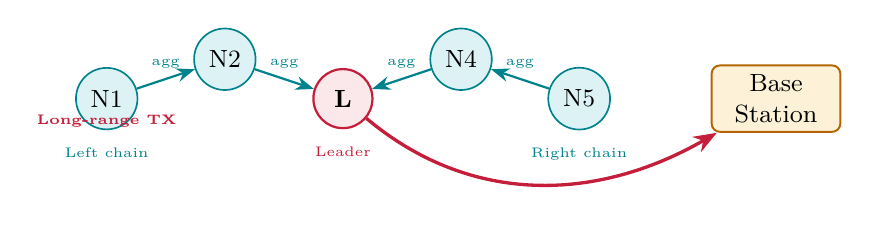
\begin{tikzpicture}[node distance=0.3cm,
  cnode/.style={circle, draw=myteal, fill=hdrteal, minimum size=0.75cm, font=\small, line width=0.6pt},
  lnode/.style={circle, draw=myred, fill=hdrred, minimum size=0.75cm, font=\small\bfseries, line width=0.8pt},
  bsnode/.style={rectangle, draw=myamber, fill=hdramber, text width=1.4cm, align=center, minimum height=0.75cm, font=\small, rounded corners=3pt, line width=0.7pt}]

  % Chain nodes
  \node[cnode] (n1) at (0,0)   {N1};
  \node[cnode] (n2) at (1.5,0.5) {N2};
  \node[lnode] (n3) at (3.0,0)  {L};
  \node[cnode] (n4) at (4.5,0.5) {N4};
  \node[cnode] (n5) at (6.0,0) {N5};
  \node[bsnode] (bs) at (8.5,0) {Base Station};

  % Chain links
  \draw[arrow, color=myteal] (n1) -- (n2) node[midway, above, font=\tiny] {agg};
  \draw[arrow, color=myteal] (n2) -- (n3) node[midway, above, font=\tiny] {agg};
  \draw[arrow, color=myteal] (n5) -- (n4) node[midway, above, font=\tiny] {agg};
  \draw[arrow, color=myteal] (n4) -- (n3) node[midway, above, font=\tiny] {agg};
  \draw[redarrow, line width=1.2pt] (n3) to[out=-40, in=210] (bs) node[midway, below=2pt, font=\tiny\bfseries, color=myred] {Long-range TX};

  \node[font=\tiny, color=myred, below=0.1cm of n3] {Leader};
  \node[font=\tiny, color=myteal, below=0.1cm of n1] {Left chain};
  \node[font=\tiny, color=myteal, below=0.1cm of n5] {Right chain};
\end{tikzpicture}
\end{tcolorbox}

\textbf{PEGASIS vs LEACH:}

\par\noindent
{\renewcommand{\arraystretch}{1.5}%
\begin{tabularx}{\linewidth}{|B{3.0cm}|Y|Y|}
\hline
\textbf{Parameter} & \textbf{LEACH} & \textbf{PEGASIS} \\
\hline
\textbf{Structure} & Clusters with CH & Single chain of all nodes \\
\hline
\textbf{Aggregation} & At CH only & Along entire chain (progressive) \\
\hline
\textbf{Transmission} & CH to BS (one-hop) & Leader to BS (one-hop) \\
\hline
\textbf{Energy balance} & Good (CH rotation) & Better (all nodes in chain share load) \\
\hline
\textbf{Latency} & Lower & Higher (data propagates along chain) \\
\hline
\textbf{Complexity} & Moderate & Higher (global chain construction) \\
\hline
\end{tabularx}}

\subsection{Data Aggregation and Fusion}

\begin{tcolorbox}[defbox, title={\textbf{Data Aggregation / Fusion --- Definition}}]
\textbf{Data aggregation} (also called \textbf{data fusion}) is the process of combining raw sensor readings from multiple nodes into a \textbf{single, compact, representative value} at an intermediate node (cluster head or relay) before forwarding to the base station. It reduces the volume of data transmitted, saving energy and bandwidth.
\end{tcolorbox}

\subsubsection*{Types of Data Aggregation}

\par\noindent
{\renewcommand{\arraystretch}{1.5}%
\begin{tabularx}{\linewidth}{|B{3.0cm}|Y|Y|}
\hline
\textbf{Type} & \textbf{Description} & \textbf{Example} \\
\hline
\textbf{Lossless aggregation} & Data combined without information loss & Concatenation, exact sum \\
\hline
\textbf{Lossy aggregation} & Data reduced with acceptable information loss & Average, max, min, median \\
\hline
\textbf{In-network processing} & Computation done at intermediate nodes, not just the sink & Cluster-head averaging in LEACH \\
\hline
\textbf{Suppression} & Nodes suppress transmission if reading is similar to a previous one (no change) & Temperature monitoring with dead-band \\
\hline
\end{tabularx}}

\subsubsection*{Common Aggregation Functions}
\begin{itemize}[leftmargin=*, itemsep=2pt]
  \item \textbf{MAX/MIN:} Forward the maximum or minimum of all received values. Used in intrusion detection.
  \item \textbf{SUM:} Total of all readings. Used in counting applications.
  \item \textbf{AVERAGE:} Mean of all readings. Used in temperature/environmental monitoring.
  \item \textbf{COUNT:} Number of nodes reporting. Used for density estimation.
  \item \textbf{Duplicate elimination:} Discard packets received from multiple paths with the same sequence number.
\end{itemize}

\textbf{Energy savings from aggregation:} If $k$ nodes each generate $b$ bits, naive forwarding requires $k \cdot b$ bits at the sink. Aggregating to a single message of $b$ bits reduces traffic by factor $k$ --- significant for large $k$.

% ===============================================================================
\section{Quality of a Sensor Network}
% ===============================================================================

\begin{tcolorbox}[formulabox, title={\textbf{QoS Metrics for WSN}}]
\begin{enumerate}[leftmargin=*, itemsep=5pt]
  \item \textbf{Energy efficiency / Network lifetime:} The most important metric. Lifetime = time until first (or $k$-th) node depletes its energy. Measured in hours or days.

  \item \textbf{Coverage:} Fraction of the monitored area where at least one sensor node can sense events. Full coverage $\Rightarrow$ every point in the field has a sensor within sensing radius $r_s$.

  \item \textbf{Connectivity:} The network is connected if there exists a path from every node to the sink. Requires $r_c \geq r_s$ (communication radius $\geq$ sensing radius).

  \item \textbf{Latency (Delay):} Time from event occurrence to data reaching the sink. Critical for real-time applications (fire detection, intruder alarm).

  \item \textbf{Reliability / Packet delivery ratio (PDR):} Fraction of generated data packets that are correctly received at the sink. $\text{PDR} = \frac{\text{received}}{\text{generated}}$

  \item \textbf{Data freshness:} How recent the received data is. Fresh data has small timestamp age.

  \item \textbf{Scalability:} Performance should degrade gracefully as node count increases from 10 to 10,000.

  \item \textbf{Fault tolerance:} Continued operation despite node or link failures.
\end{enumerate}
\end{tcolorbox}

\subsection{Real-Time Traffic Support in WSN}

Real-time applications (e.g., structural collapse detection, fire alarm) require end-to-end delay guarantees.

\begin{itemize}[leftmargin=*, itemsep=3pt]
  \item \textbf{Priority queuing:} High-priority (alarm) packets bypass normal queue.
  \item \textbf{Multi-path routing:} Maintain multiple paths; switch to backup on congestion.
  \item \textbf{Guaranteed Time Slots (GTS) in IEEE 802.15.4:} CFP slots are collision-free and schedule-based --- provides bounded latency.
  \item \textbf{SPEED protocol:} Stateless, geographic routing protocol designed for real-time traffic in WSN. Each node maintains a desired forwarding speed; if current speed is insufficient, the packet is re-routed.
  \item \textbf{Queue management:} Drop tail, RED (Random Early Detection), or priority-based scheduling at each relay node.
\end{itemize}

% ===============================================================================
\section{Security in Wireless Sensor Networks}
% ===============================================================================

WSN security is challenging because nodes are \textbf{physically exposed} in the field and have \textbf{very limited resources} for cryptographic computations.

\subsection{Security Goals (CIA + More)}

\begin{tcolorbox}[examplebox, title={\textbf{Security Goals in WSN}}]
\begin{itemize}[leftmargin=*, itemsep=4pt]
  \item \textbf{Confidentiality:} Only authorized parties can read the data. Achieved by symmetric encryption (AES).
  \item \textbf{Integrity:} Data is not modified in transit. Achieved by Message Authentication Codes (MAC).
  \item \textbf{Authentication:} Data genuinely comes from the claimed source. Achieved by keyed-hash MACs.
  \item \textbf{Availability:} The network remains operational despite attacks (anti-jamming, redundancy).
  \item \textbf{Freshness:} Data is recent, not a replay. Achieved by nonces, counters, or timestamps.
  \item \textbf{Self-organization:} Nodes can re-key and reform the network if a node is compromised.
\end{itemize}
\end{tcolorbox}

\subsection{Attack Types in WSN}

\par\noindent
{\renewcommand{\arraystretch}{1.5}%
\begin{tabularx}{\linewidth}{|B{3.0cm}|Y|Y|}
\hline
\textbf{Attack} & \textbf{Description} & \textbf{Defense} \\
\hline
\textbf{Sybil attack} & A malicious node presents multiple fake identities to the network & Identity-based authentication, physical challenge \\
\hline
\textbf{Wormhole attack} & Attacker tunnels packets between two distant points out-of-band, creating a fake short-cut & Geographic routing, TIK (time-based packet leash) \\
\hline
\textbf{Selective forwarding} & A malicious node drops selected packets instead of forwarding them all & Multi-path routing, ACK-based detection \\
\hline
\textbf{DoS (Jamming)} & Attacker transmits RF noise to block legitimate communication & Frequency hopping, spread spectrum (DSSS) \\
\hline
\textbf{Sinkhole attack} & A compromised node advertises a falsely attractive route to pull all traffic through itself & Geographic + authenticated routing \\
\hline
\textbf{Hello flood attack} & Attacker broadcasts HELLO packets with high power; distant nodes think it's a neighbor & Bidirectional link verification \\
\hline
\textbf{Replay attack} & Attacker captures a valid packet and retransmits it later & Timestamps, nonces, counters \\
\hline
\textbf{Node capture} & Physically capturing a node to extract keys & Key pre-distribution, threshold schemes \\
\hline
\end{tabularx}}

\subsection{SPINS: Security Protocols for Sensor Networks}

\begin{tcolorbox}[defbox, title={\textbf{SPINS --- Definition}}]
\textbf{SPINS (Security Protocols for Sensor Networks)} is a security framework for WSN that provides two building blocks:
\begin{itemize}
  \item \textbf{SNEP (Sensor Network Encryption Protocol):} Provides data confidentiality, data authentication, and data freshness between sensor nodes and base station.
  \item \textbf{\boldmath$\mu$TESLA (micro Timed Efficient Stream Loss-tolerant Authentication):} Provides \textbf{authenticated broadcast} from base station to sensor nodes using delayed key disclosure.
\end{itemize}
\end{tcolorbox}

\subsubsection*{SNEP Features}

\begin{itemize}[leftmargin=*, itemsep=3pt]
  \item Uses a shared symmetric key between each node and the base station (established at deployment).
  \item \textbf{Confidentiality:} Data encrypted with a block cipher (AES in counter mode).
  \item \textbf{Data authentication:} A MAC (Message Authentication Code) is appended to each message.
  \item \textbf{Freshness:} A counter (nonce) is included; base station checks that counter is monotonically increasing, preventing replay attacks.
  \item \textbf{Low overhead:} Counter is shared state; only 2 bytes added per packet for freshness (not a full timestamp).
\end{itemize}

\subsubsection*{\texorpdfstring{$\mu$}{mu}TESLA: Authenticated Broadcast}

Standard MACs require the receiver to share the key with the sender. In broadcast, if the key is shared with all receivers, any malicious receiver can forge messages. $\mu$TESLA solves this with \textbf{delayed key disclosure}:

\begin{enumerate}[leftmargin=*, itemsep=3pt]
  \item Base station generates a one-way key chain: $K_n, K_{n-1}, \ldots, K_1, K_0$ where $K_{i-1} = H(K_i)$ (hash function).
  \item Publishes commitment $K_0$ to all nodes at deployment.
  \item To broadcast a packet in time interval $i$: append MAC using $K_i$ (key not yet revealed).
  \item After the time interval passes, base station \textbf{discloses} $K_i$ to all nodes.
  \item Nodes verify the disclosed key (check $H(K_i) = K_{i-1}$) and then authenticate the buffered packet.
\end{enumerate}

\begin{tcolorbox}[tikzbox, title={\texorpdfstring{$\mu$}{mu}TESLA Key Chain and Delayed Disclosure}]
\centering
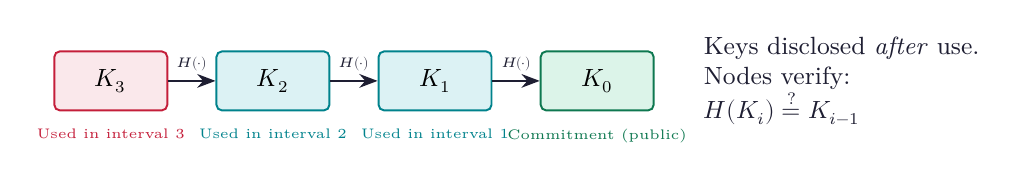
\begin{tikzpicture}[node distance=0.2cm,
  knode/.style={rectangle, draw=myteal, fill=hdrteal, text width=1.2cm, align=center, minimum height=0.75cm, font=\small\bfseries, rounded corners=2pt, line width=0.7pt}]

  \node[knode, fill=hdrred, draw=myred] (k3) {$K_3$};
  \node[knode, right=0.6cm of k3] (k2) {$K_2$};
  \node[knode, right=0.6cm of k2] (k1) {$K_1$};
  \node[knode, right=0.6cm of k1, fill=hdrgreen, draw=mygreen] (k0) {$K_0$};

  \draw[arrow] (k3) -- (k2) node[midway, above, font=\tiny] {$H(\cdot)$};
  \draw[arrow] (k2) -- (k1) node[midway, above, font=\tiny] {$H(\cdot)$};
  \draw[arrow] (k1) -- (k0) node[midway, above, font=\tiny] {$H(\cdot)$};

  \node[font=\tiny, color=myred, below=0.1cm of k3] {Used in interval 3};
  \node[font=\tiny, color=myteal, below=0.1cm of k2] {Used in interval 2};
  \node[font=\tiny, color=myteal, below=0.1cm of k1] {Used in interval 1};
  \node[font=\tiny, color=mygreen, below=0.1cm of k0] {Commitment (public)};

  \node[right=0.5cm of k0, font=\small, color=mydark, align=left]
    {Keys disclosed \textit{after} use.\\ Nodes verify:\\$H(K_i) \stackrel{?}{=} K_{i-1}$};
\end{tikzpicture}
\end{tcolorbox}

\subsection{Key Management in WSN}

\begin{itemize}[leftmargin=*, itemsep=3pt]
  \item \textbf{Pre-deployment key loading:} Each node gets a unique secret key shared with the base station.
  \item \textbf{Random key pre-distribution (Eschenauer-Gligor):} Each node pre-loaded with a random subset of keys from a large key pool. Two neighboring nodes likely share at least one key (used for pairwise link encryption).
  \item \textbf{Threshold-based schemes:} A secret key is split into $n$ shares using Shamir's Secret Sharing; any $k$ out of $n$ nodes can reconstruct the key.
\end{itemize}

% ===============================================================================
\newpage
\begin{center}
  {\large\bfseries\color{myred} Quick Revision --- Module 4}\\[3pt]
  {\small\color{mydark} Dissemination, Data Fusion, QoS \& Security $|$ PE-EC703B}
\end{center}
\noindent{\color{myred}\rule{\linewidth}{1.2pt}}
\vspace{4pt}
% ===============================================================================

\begin{tcolorbox}[formulabox, title={\textbf{Key Formulas and Metrics at a Glance}}]
\renewcommand{\arraystretch}{1.35}
\begin{tabularx}{\linewidth}{B{5.0cm} X}
Packet Delivery Ratio & $\text{PDR} = \displaystyle\frac{\text{Packets received at sink}}{\text{Packets generated at source}} \times 100\%$ \\[6pt]
Network Lifetime & $T = \displaystyle\min_i \left(\frac{E_i}{P_i}\right)$ \quad (limited by first node to die) \\[6pt]
Sensing Coverage Area & $C = \displaystyle\frac{\text{Sensed area}}{\text{Total monitored area}}$ \quad (per-node area $= \pi r_s^2$) \\[6pt]
Aggregation Energy Saved & $E_{\text{saved}} = (k-1) \times b \times E_{\text{tx/bit}}$ \quad (for $k$ streams aggregated) \\[6pt]
$\mu$TESLA Verification & $K_{i-1} = H(K_i)$ \quad (verify: $H(K_{\text{disclosed}}) = K_{\text{prev}}$)
\end{tabularx}
\end{tcolorbox}

\begin{tcolorbox}[defbox, title={\textbf{One-Line Definitions}}]
\begin{itemize}[leftmargin=*, itemsep=3pt]
  \item \textbf{Data dissemination:} Propagating data or queries across WSN from source to destination with energy efficiency.
  \item \textbf{Rumor routing:} Agents wander creating routing tables; queries find event by intersecting agent trails.
  \item \textbf{PEGASIS:} Chain-based data gathering; data aggregated node-by-node to leader, then to base station.
  \item \textbf{Data aggregation:} Combining multiple sensor readings into a single compact value to save transmission energy.
  \item \textbf{Sybil attack:} Malicious node uses multiple fake identities to influence routing or voting.
  \item \textbf{Wormhole attack:} Attacker tunnels packets out-of-band to create a false short-cut route.
  \item \textbf{SPINS:} Security framework for WSN comprising SNEP (confidentiality/authentication) and $\mu$TESLA (authenticated broadcast).
  \item \textbf{$\mu$TESLA:} Authenticated broadcast via delayed key disclosure from a one-way key chain.
\end{itemize}
\end{tcolorbox}

\begin{tcolorbox}[exambox, title={\textbf{Frequently Asked / Viva Questions}}]
\begin{enumerate}[topsep=0pt, label=\textbf{Q\arabic*.}, itemsep=5pt]
  \item \Q{What is data dissemination in WSN? Name two dissemination protocols.}
  Data dissemination is the mechanism by which data or queries are propagated across the WSN from source to sinks (or vice versa) efficiently. Two protocols: (1) \textbf{Directed Diffusion} --- interest flooding, gradient setup, data delivery; (2) \textbf{Rumor Routing} --- agents propagate from event sources; queries find events by intersecting agent trails.

  \item \Q{Explain data aggregation in WSN. What are its benefits?}
  Data aggregation combines sensor readings from multiple nodes into a single compact value at an intermediate node before forwarding to the sink. Benefits: (1) Reduces data volume $\Rightarrow$ fewer transmissions $\Rightarrow$ energy savings; (2) Reduces congestion; (3) Eliminates redundant data from correlated sensors.

  \item \Q{What is PEGASIS? How is it better than LEACH?}
  PEGASIS (Power-Efficient GAthering in Sensor Information Systems) forms a single chain of all nodes; data is aggregated along the chain to a rotating leader that transmits to the base station. Better than LEACH because: (1) Progressive in-network aggregation reduces total data volume; (2) Each node only communicates with its nearest neighbor (shorter range $\Rightarrow$ less energy); (3) Leader rotation distributes the high-energy BS transmission among all nodes.

  \item \Q{List four QoS metrics for a wireless sensor network.}
  (1) \textbf{Network lifetime} --- time until first node dies; (2) \textbf{Coverage} --- fraction of area monitored; (3) \textbf{Latency} --- delay from event to sink; (4) \textbf{PDR (Packet Delivery Ratio)} --- fraction of packets successfully received.

  \item \Q{What is the Sybil attack and how is it prevented?}
  In a Sybil attack, a malicious node presents multiple fake identities to the network, allowing it to manipulate routing decisions, vote-based algorithms, or reputation systems. Prevention: (1) Identity-based authentication (each node has a unique certificate); (2) Physical challenge tests (test if a ``node'' is actually at its claimed location); (3) Radio fingerprinting.

  \item \Q{Explain the wormhole attack and its impact on WSN.}
  Two colluding attackers at distant parts of the network create a private, out-of-band tunnel (wormhole). Packets received by one end are instantly forwarded to the other end, making distant nodes appear as neighbors. This distorts routing: nodes route via the wormhole (thinking it is a short path), allowing attackers to eavesdrop or drop packets. Countermeasures: TIK (timestamp-based packet leash), geographic routing with location verification.

  \item \Q{What is SPINS? Explain SNEP.}
  SPINS (Security Protocols for Sensor Networks) provides two security primitives. \textbf{SNEP} (Sensor Network Encryption Protocol) provides: confidentiality (AES counter-mode encryption), data authentication (keyed MAC), and freshness (shared counter prevents replay). Low overhead: only 8 bytes MAC per packet. SNEP uses pairwise shared keys between each node and the base station.

  \item \Q{How does $\mu$TESLA provide authenticated broadcast?}
  $\mu$TESLA uses a \textbf{one-way key chain}: $K_{i-1} = H(K_i)$, bootstrapped with commitment $K_0$ published to all nodes. For interval $i$, base station authenticates broadcast with $K_i$ (key still secret). After the interval ends, $K_i$ is disclosed. Nodes verify: $H(K_i) \stackrel{?}{=} K_{i-1}$. If valid, they authenticate the earlier buffered message. Delayed disclosure ensures receivers cannot forge the MAC.

  \item \Q{What is selective forwarding attack in WSN?}
  A malicious intermediate node drops specific packets instead of forwarding them all. It behaves correctly for some flows to avoid detection. Impact: data loss, reduced PDR, silent disruption of critical sensor data. Defense: multi-path routing ensures data reaches sink via alternative paths; ACK-based detection flags suspicious forwarders.

  \item \Q{What is real-time traffic support in WSN?}
  Applications like fire alarms or structural collapse detection require end-to-end delay guarantees. Mechanisms: (1) \textbf{Priority queuing} at routers for alarm packets; (2) \textbf{GTS slots} in IEEE 802.15.4 (collision-free, bounded delay); (3) \textbf{SPEED protocol} --- geographic routing enforcing minimum forwarding speed; (4) Multi-path routing for congestion avoidance.

  \item \Q{Differentiate data gathering and data dissemination.}
  \textbf{Data gathering} = collecting sensor readings from nodes to the base station (many-to-one, uplink). \textbf{Data dissemination} = propagating queries or commands from sink to sensor nodes, or flooding data from a source to multiple sinks (one-to-many or controlled spreading). Gathering protocols: PEGASIS, LEACH. Dissemination protocols: Directed Diffusion, Rumor Routing, SPIN.

  \item \Q{What is the Hello flood attack?}
  An attacker with a powerful radio broadcasts HELLO messages at high power. Nodes far away hear this and assume the attacker is a one-hop neighbor, establishing routes through it. When they try to send data via this ``neighbor,'' packets are lost or intercepted. Defense: bidirectional link verification --- a node only considers a neighbor if it can receive a reply from that neighbor at normal power.
\end{enumerate}
\end{tcolorbox}

\begin{tcolorbox}[tikzbox, title={\textbf{Summary: WSN Security Threats and Countermeasures}}]
\par\noindent
{\renewcommand{\arraystretch}{1.4}%
\begin{tabularx}{\linewidth}{|B{2.8cm}|Y|Y|}
\hline
\textbf{Attack} & \textbf{Layer} & \textbf{Countermeasure} \\
\hline
Sybil & Network & Identity auth., radio fingerprint \\
\hline
Wormhole & Network & Packet leash (TIK), location verify \\
\hline
Selective forward & Network & Multi-path, ACK detection \\
\hline
DoS / Jamming & Physical & DSSS, frequency hopping \\
\hline
Replay & MAC/Net & Nonce, timestamp, counter (SNEP) \\
\hline
Hello flood & Network & Bidirectional link verification \\
\hline
Node capture & Physical & Key pre-distribution, threshold \\
\hline
\end{tabularx}}
\end{tcolorbox}

\end{document}
